\documentclass[a4paper,11pt,dvipdfmx]{jsarticle}

\usepackage[dvipdfmx]{graphicx}
\usepackage{subcaption}
\usepackage{url}
\usepackage{bm}
\usepackage{amsmath,amssymb}
\usepackage{ascmac}

%\captionsetup[subfigure]{labelformat=simple}
\renewcommand{\thesubfigure}{(\alph{subfigure})}

\newcommand{\qed}{\hfill$\Box$}
\newcommand{\Proof}{\noindent{\bf Proof.}\quad}
\makeatletter
\newcommand{\figcaption}[1]{\def\@captype{figure}\caption{#1}}
\newcommand{\tblcaption}[1]{\def\@captype{table}\caption{#1}}
\makeatother

\newcommand{\bhline}[1]{\noalign{\hrule height #1}}  
\newcommand{\bvline}[1]{\vrule width #1}  

\begin{document}

\title{\vspace{-2cm}クラスター分析}
\author{富島諒}
\date{\today}

\maketitle
\section{クラスター分析}
\subsection*{クラスター分析とは}
\label{sec:cluster}
クラスタとは, "群れ"や"集団"という意味を持つ. そして, クラスター分析とは, 与えられたデータを"似たものどうしの群れに分ける方法"である. クラスター分析ではデータのことを"個体"と呼び, 個体と個体とが集まって, クラスタを構成することになる. 

しかし, このままではクラスタに分類する基準が曖昧であるため, "似ている"とは何かを数学的に定義する必要がある. そこでまず, "似ている程度"を測る方法として, 以下のようなものがあげられる. 
\[
  \left\{
    \begin{tabular}{l}
      ユークリッド距離 \\
      ユークリッド距離の2乗 \\
      マハラノビスの距離 \\
      相関係数
    \end{tabular}
  \right.
\]
これらの方法は, 距離の概念を一般化したものと考えられるので, これらを広い意味で"距離"と呼ぶこととする. 

\subsection*{クラスタ間の距離}
分析の際, "2つのクラスタ間の距離$D$をどのように決めるか"という問題が発生する. もし, 各クラスタの成分が1個だけならば, 個体間の距離をそのまま$D$とすればよい. では, 各クラスタの成分が2個以上から成る場合は, どのように距離$D$を測ればよいだろうか? (図\ref{fig:cluster_diff})

\begin{figure}[htb]
  \centering
  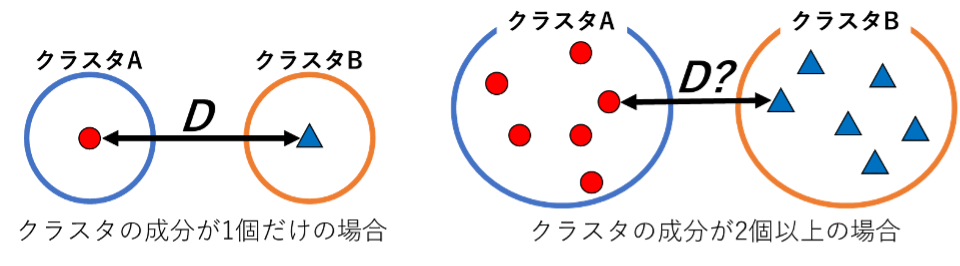
\includegraphics[width=14cm]{../pics/cluster_1or.png}
  \caption{成分の個数によるクラスタ分析の違い}
  \label{fig:cluster_diff}
\end{figure}

この"2つのクラスタ間の距離$D$の決め方"には, 多くの方法が存在しており, $\S2$では, そのうちの6つの手法について説明する. 

\section{クラスタ間の距離の決め方}
\label{sec:how_to_decide}

\subsection*{最短距離法}
クラスタAの個体とクラスタBの個体とのすべての組み合わせについて距離を求め, 
その中で最も短い距離をクラスタ間の距離$D$と定義する. (図\ref{fig:sdm})

\begin{figure}[htb]
  \centering
  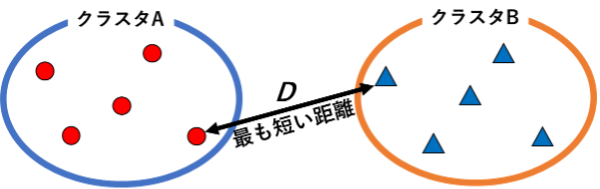
\includegraphics[width=8cm]{../pics/SDM.png}
  \caption{最短距離法}
  \label{fig:sdm}
\end{figure}

\subsection*{最長距離法}
クラスタAの個体とクラスタBの個体とのすべての組み合わせについて距離を求め, 
その中で最も長い距離をクラスタ間の距離$D$と定義する. (図\ref{fig:ldm})

\begin{figure}[htb]
  \centering
  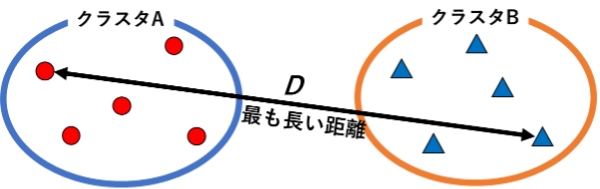
\includegraphics[width=8cm]{../pics/LDM.png}
  \caption{最長距離法}
  \label{fig:ldm}
\end{figure}

\subsection*{群平均法}
クラスタAの個体とクラスタBの個体との全ての組み合わせについて距離を求め, 
その距離の平均値をクラスタ間の距離$D$と定義する. (図\ref{fig:gam})

\begin{figure}[htb]
  \centering
  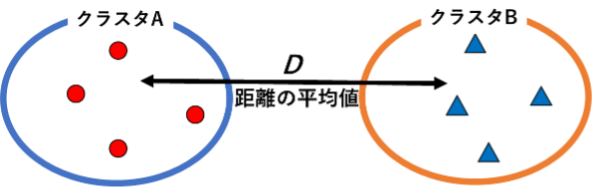
\includegraphics[width=8cm]{../pics/GAM.png}
  \caption{群平均法}
  \label{fig:gam}
\end{figure}

\subsection*{メディアン法}
クラスタAの個体とクラスタBの個体との全ての組み合わせについて距離を求め, 
その距離を順番に並べたときの中央値(メディアン)をクラスタ間距離$D$と定義する. (図\ref{fig:med})

\begin{figure}[htb]
  \centering
  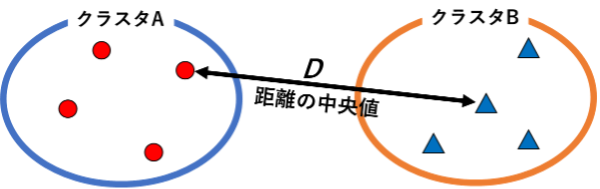
\includegraphics[width=8cm]{../pics/MED.png}
  \caption{メディアン法}
  \label{fig:med}
\end{figure}

\subsection*{重心法}
クラスタAの重心とクラスタBの重心との距離を, クラスタ間距離$D$と定義する. (図\ref{fig:center})

\begin{figure}[htb]
  \centering
  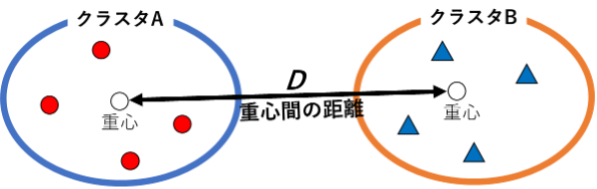
\includegraphics[width=8cm]{../pics/Center.png}
  \caption{重心法}
  \label{fig:center}
\end{figure}

\subsection*{ウォード法}
例えば, シャムネコとペルシャネコをまとめてネコたちと呼んでしまうと, もともとどんなネコいたのかわからなくなってしまう. このように, 異なるものを1つにまとめると,元の情報が少し失われて しまう. これをクラスタの情報損失量と呼ぶこととする.

ウォード法では, 2つのクラスタA, Bを1つのクラスタにまとめたとき, その情報損失量をクラスタ間の距離$D$とする. (図\ref{fig:ward})

\begin{figure}[htb]
  \centering
  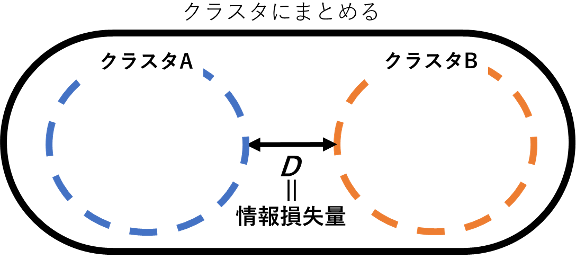
\includegraphics[width=8cm]{../pics/Ward.png}
  \caption{ウォード法}
  \label{fig:ward}
\end{figure}

具体的に, クラスタ間の距離$D$は, 以下のような式で定義される. 
\[
  クラスタ間の距離D = L(A\cup B) -L(A) - L(B)
\]
ここで$L(A)$は, クラスタAの各個体から重心までの距離の2乗和を計算したもので, クラスタ内でのデータの散らばり具合を表現している. $L(B)$及び$L(A\cup B)$同様である. 

\section{クラスター分析の手順}
\label{sec:method_of_cluster}
表\ref{tab:aids}のデータを使って, 実際にクラスター分析をしてみる. クラスター分析は, 以降のような手順で進んでいき, 次々にまとまっていくクラスタをデンドログラム(樹形図)というグラフで表現する. なお今回, 距離は平方ユークリッド距離, クラスタ間距離は重心法を用いて求めていく. 

\begin{table}[htb]
  \centering
  \caption{エイズ患者数と新聞の発行部数}
  \label{tab:aids}
  \begin{tabular}{ccc}\bhline{1.5pt}
    国名&エイズ患者 &新聞の発行部数  \\ \hline
    A &6.6 &35.8 \\
    B &8.4 &22.1 \\
    C &24.2&19.1 \\
    D &10.0&34.4 \\
    E &14.5&9.9 \\
    F &12.2&31.1 \\
    G &4.8 &53.0 \\
    H &19.8&7.5 \\
    I &6.1 &53.4\\
    J &26.8&50.0\\
    K &7.4 &42.1\\ \hline
  \end{tabular}
\end{table}

\begin{figure}[htb]
  \centering
  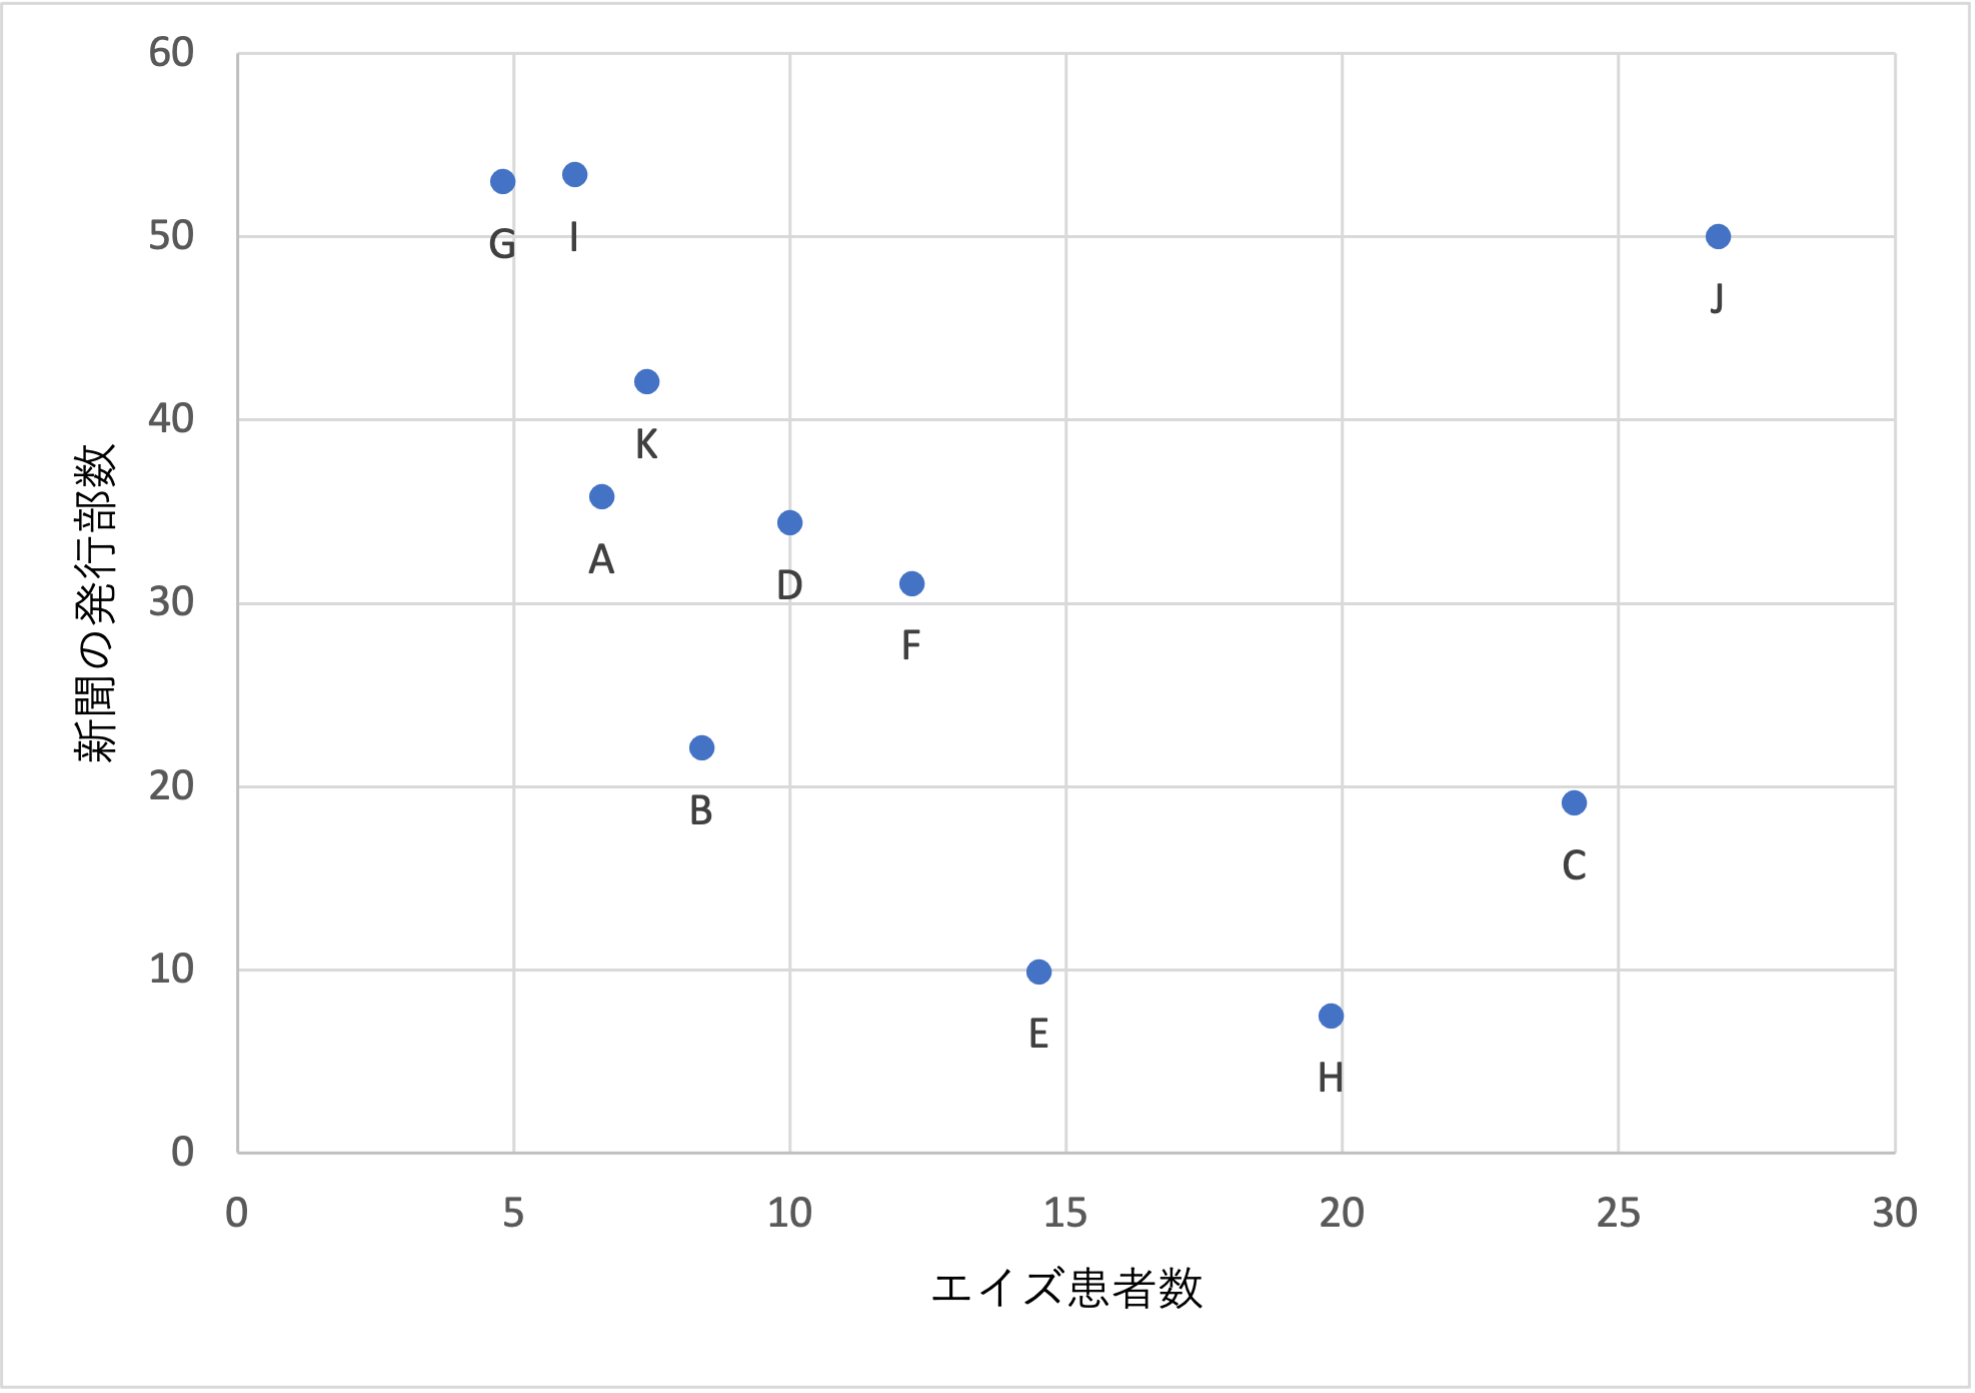
\includegraphics[width=10cm]{../pics/aids.png}
  \caption{エイズ患者数と新聞の発行部数}
  \label{fig:aids_and_circulation}
\end{figure}

\subsubsection*{手順1}
はじめに, すべての組み合わせにおける"距離"を計算すると, 以下の表\ref{tab:initial_distance}のようになる. 

\begin{figure}[htb]
  \centering
  \tblcaption{手順1による距離の計算結果}
  \label{tab:initial_distance}
  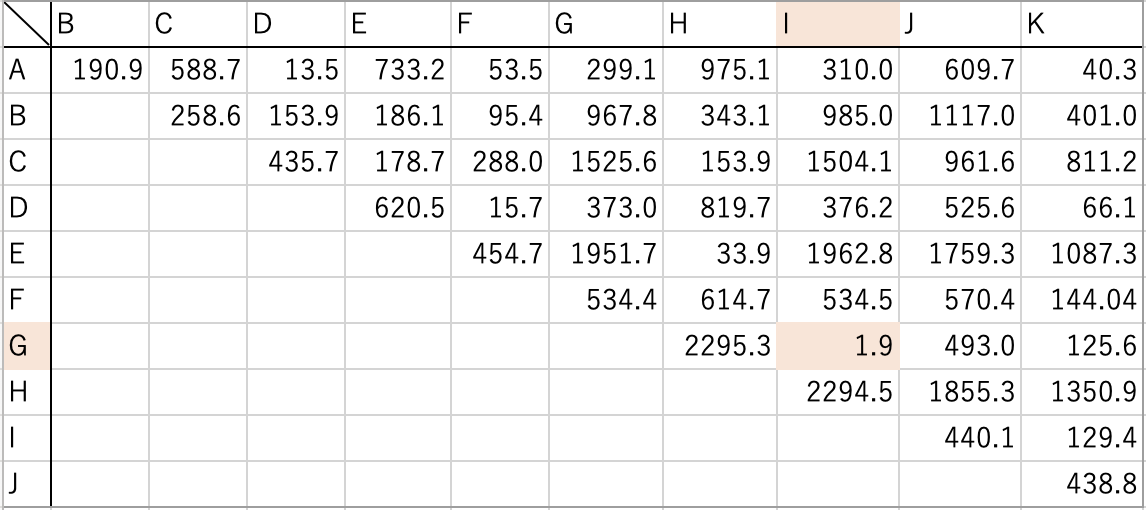
\includegraphics[width=10cm]{../pics/tab1.png}
\end{figure}

この中で, GとIの間の距離が
\[
  (4.8-6.1)^2+(53.0-53.4)^2=1.85 \simeq 1.9
\]
となり, すべての組み合わせの中で最小になる. よって, GとIが最初のグラスタ\{G, I\}を構成する. これをデンドログラムに描くと, 図\ref{fig:dendro1}のようになる. 

\begin{figure}[htb]
  \centering
  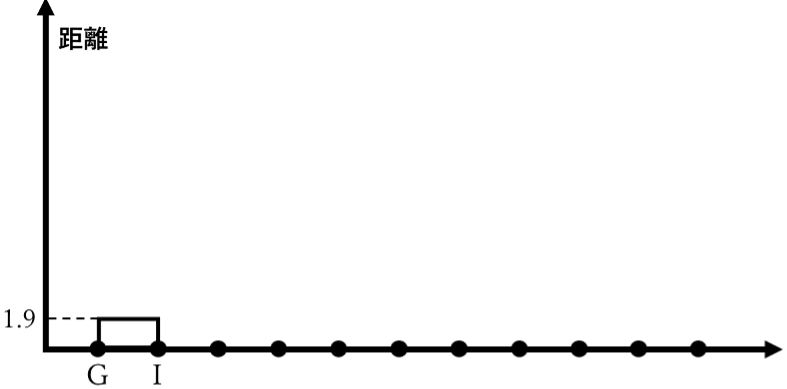
\includegraphics[width=10cm]{../pics/dendro_1.png}
  \caption{手順1によるデンドログラム}
  \label{fig:dendro1}
\end{figure}

また, クラスタ\{G, I\}の重心を求めると(5.45, 53.2)であり, 以降の手順ではこの重心を基点として, クラスタ\{G, I\}との距離を計算していく. 

%\clearpage

\subsubsection*{手順2}
次に残りすべての組み合わせにおける"距離"を計算すると, 以下の表\ref{tab:seconde_distance}のようになる. 

\begin{figure}[htb]
  \centering
  \tblcaption{手順2による距離の計算結果}
  \label{tab:seconde_distance}
  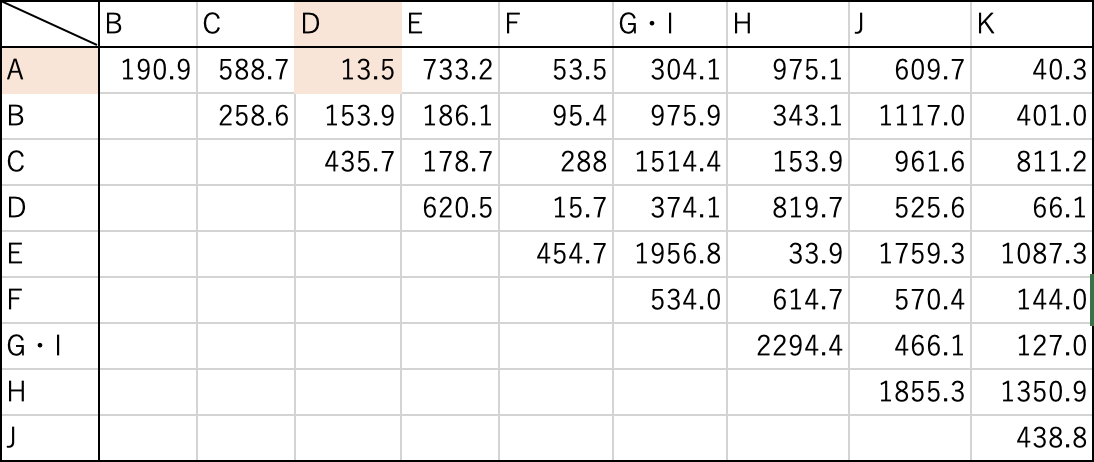
\includegraphics[width=10cm]{../pics/tab2.png}
\end{figure}

この中でAとDの組み合わせが最小となる. よって, AとDが2つ目のクラスタ\{A, D\}を構成する. これをデンドログラムに描き加えると, 図\ref{fig:dendro2}のようになる. 

\begin{figure}[htb]
  \centering
  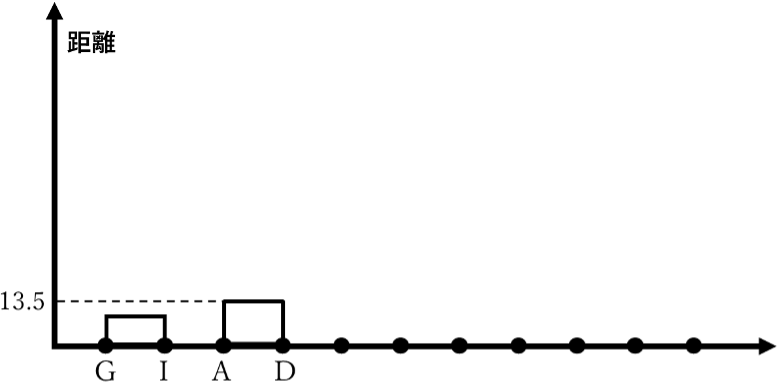
\includegraphics[width=10cm]{../pics/dendro_2.png}
  \caption{手順2によるデンドログラム}
  \label{fig:dendro2}
\end{figure}

また, クラスタ\{A, D\}の重心を求めると(8.3, 35.1)であり, 以降の手順ではこの重心を基点として, クラスタ\{A, D\}との距離を計算していく. 

\clearpage

\subsubsection*{手順3}
以上の作業を繰り返していき, 10回目で最後のクラスタが構成されて終了となる. 
最終的に完成したデンドログラムは, 次の図\ref{fig:dendro_final}のようになる. 

\begin{figure}[htb]
  \centering
  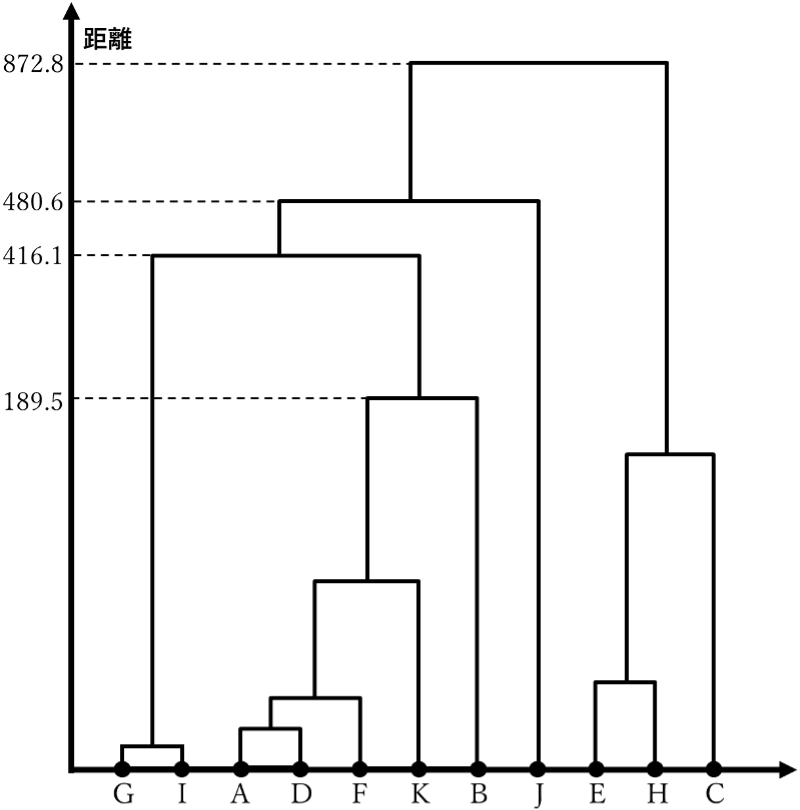
\includegraphics[width=10cm]{../pics/dendro_final.png}
  \caption{完成したデンドログラム}
  \label{fig:dendro_final}
\end{figure}

\section{デンドログラム}
\label{sec:dendrogram}
\subsection*{デンドログラムの見方}
デンドログラムは個体とクラスタ間の"距離"の関係をまとめたものであり,クラスター分析において非常に重要なグラフ表現である.

縦軸が類似度を表す"距離"となっており,横軸に平行な線を引いたとき,デンドログラムの縦線とぶつ かった個数がクラスタの個数になる. またこのとき,クラスタを構成している個体の内訳をみることが できる.

例えば, クラスタの個数を4個にしたい場合は,図\ref{fig:dendro_orange}のようにオレンジ色の平行線を引けばよい. そして,4つのクラスタはそれぞれ\{G, I\}, \{A, D, F, K, B\}, \{J\}, \{E, H, G\}という個体で構成されることが読み取れる. 

\begin{figure}[htb]
  \centering
  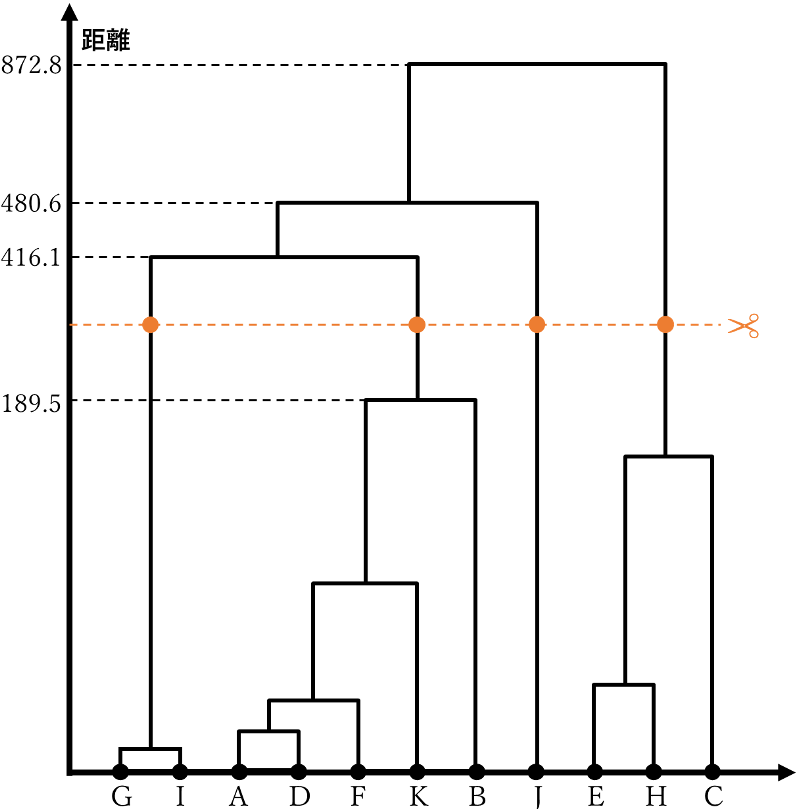
\includegraphics[width=12cm]{../pics/dendro_orange.png}
  \caption{デンドログラムを用いたクラスター分析}
  \label{fig:dendro_orange}
\end{figure}

\newpage
また, 4つのクラスタを散布図に描くと, 次の図\ref{fig:aids4}のようになる. 

\begin{figure}[htb]
  \centering
  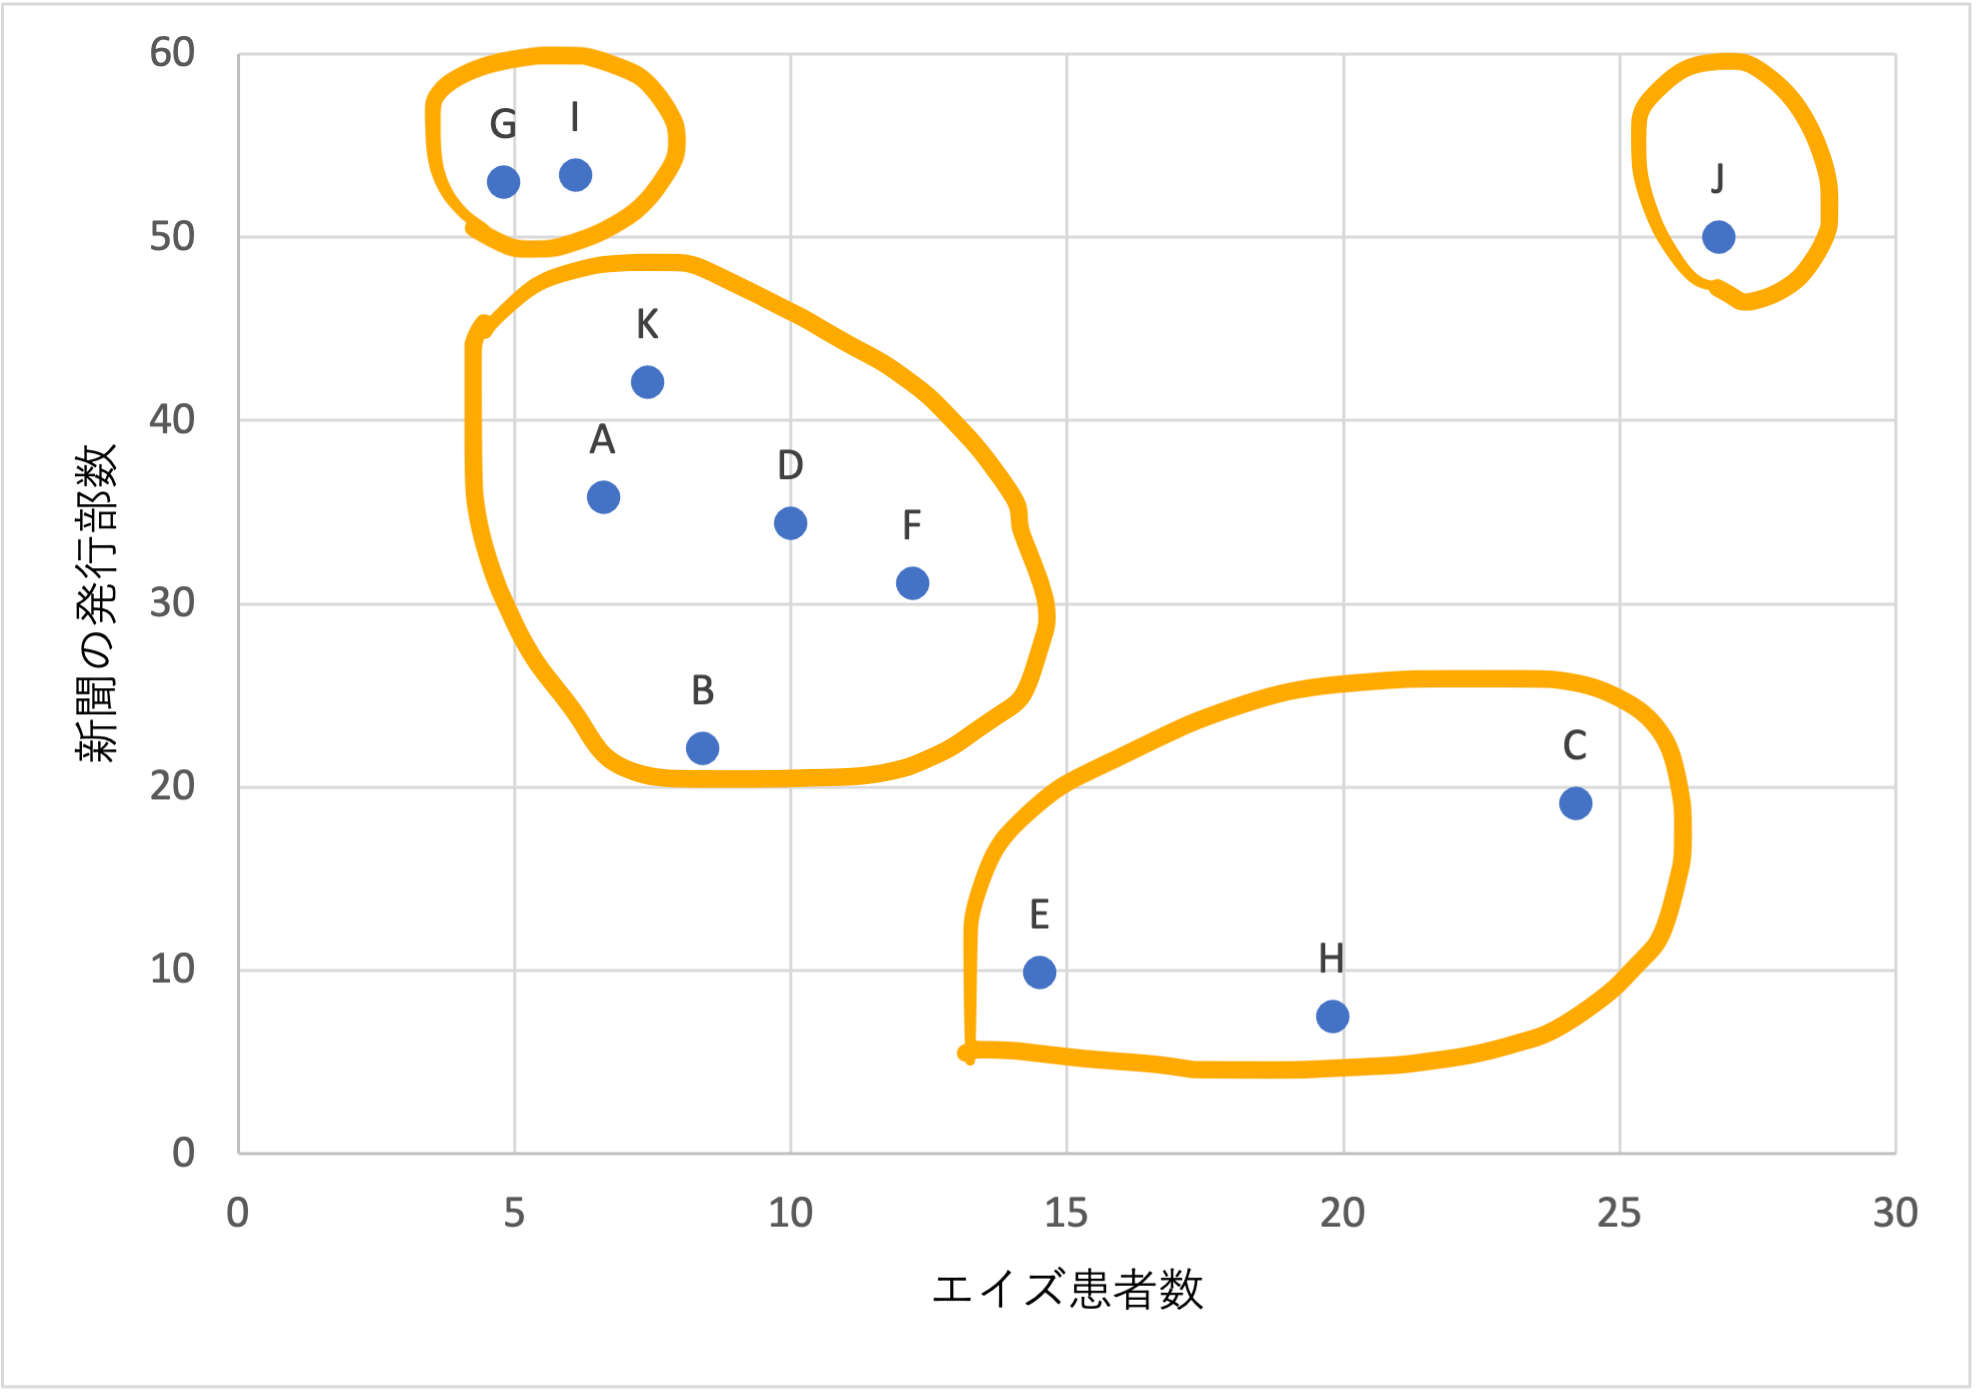
\includegraphics[width=10cm]{../pics/aids_4.png}
  \caption{クラスター分析によって4つ分類した結果}
  \label{fig:aids4}
\end{figure}

\subsection*{最適なクラスタの個数}
デンドログラムに平行線を引くことで,任意の個数のクラスタを求めることができた.
しかし,クラスター分析を行う際,"最適なクラスタの個数は何個なのか?"という問題がある. 実は, はっきりとした基準はなく,何個のクラスタに分類するかは,そのデータを研究している人次第である.

\end{document}